\subsection{Database}

Pertama kita akan membuat databasenya menggunakan MySQL. Untuk mempermudah pembuatan aplikasi kita menggunakan XAMPP yang telah berisikan Apache, MySQL, dan PHP. Jadi pastikan kalian telah menginstall XAMPP. Jika sudah, buka XAMPP kalian. Lalu jalankan Apache dan MySQL dengan mengklik start.

\begin{figure}[H]
	\centering
	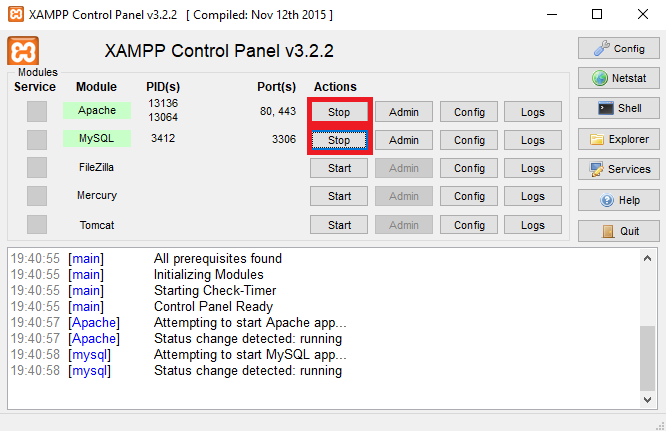
\includegraphics[width=7cm]{figures/database/database1.png}
\end{figure}

\noindent
Kemudian jalankan url http://localhost/phpmyadmin/ pada web browser kalian.

\begin{figure}[H]
\centering
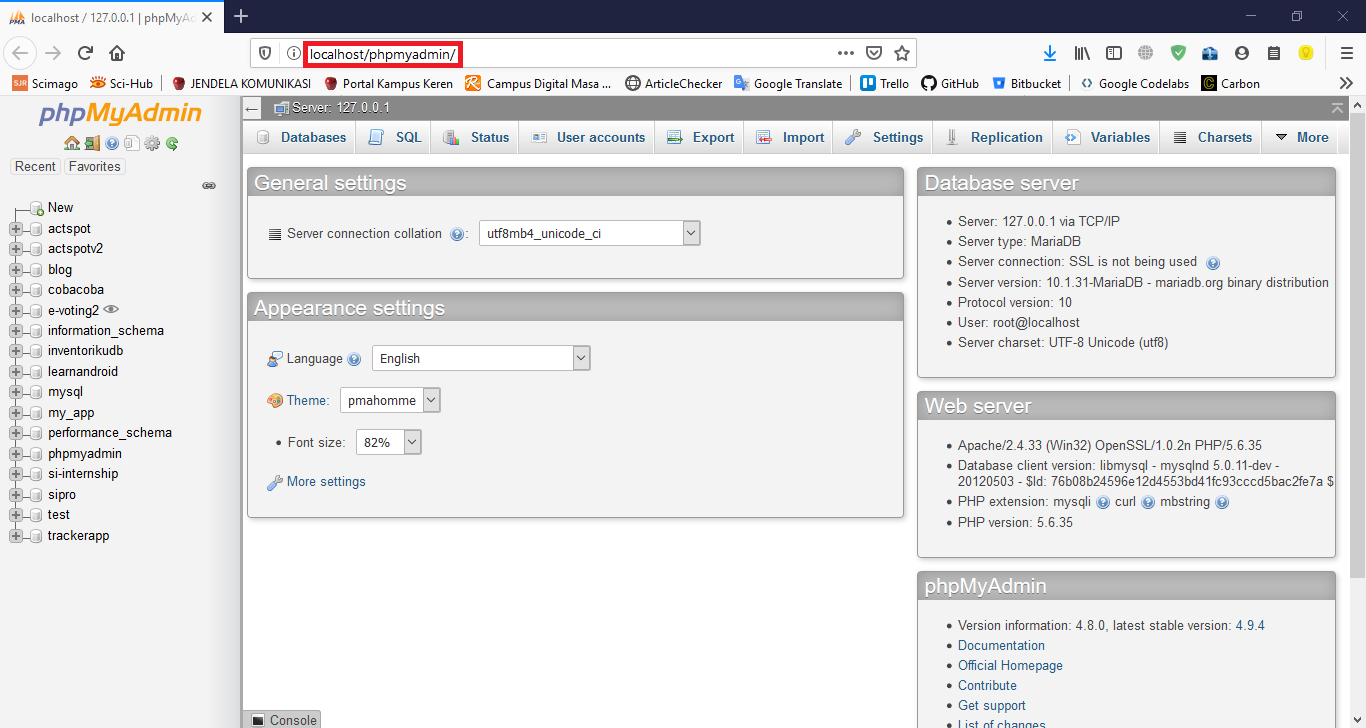
\includegraphics[width=1\textwidth]{figures/database/database2.png}
\end{figure}

\noindent
Setelah itu, kita akan membuat database dengan nama actspot. Caranya klik menu SQL, lalu ketikan script berikut. Kemudian klik Go untuk mengeksekusinya.
\begin{lstlisting}[language=SQL]
CREATE DATABASE `actspot`
\end{lstlisting}

\begin{figure}[H]
\centering
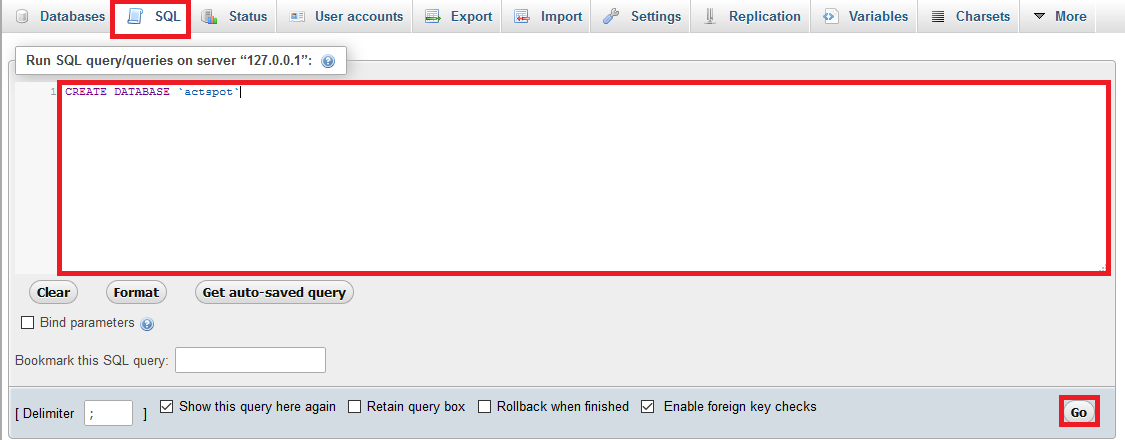
\includegraphics[width=1\textwidth]{figures/database/database3.png}
\end{figure}

\noindent
Kemudian kita buat akan membuat tabel-tabel yang nantinya dibutuhkan untuk menyimpan datanya. Caranya kita klik database yang telah dibuat sebelumnya. Setelah itu, klik menu SQL. Pertama kita akan membuat tabel absensi. Ketikan script berikut dan klik Go untuk mengeksekusinya.

\begin{lstlisting}[language=SQL]
CREATE TABLE `absensi` (
  `id_absensi` int(11) NOT NULL,
  `id_intern_absensi` varchar(10) NOT NULL,
  `id_mahasiswa_absensi` varchar(15) NOT NULL,
  `id_dosen_absensi` varchar(15) NOT NULL,
  `id_pembimbing_absensi` int(11) NOT NULL,
  `latitude_absensi` text NOT NULL,
  `longitude_absensi` text NOT NULL,
  `imei_perangkat_absensi` text NOT NULL,
  `id_kegiatan_absensi` int(11) NOT NULL,
  `catatan_absensi` text NOT NULL,
  `foto_absensi` text NOT NULL,
  `tgl_waktu_absensi` text NOT NULL,
  `status_absensi` varchar(20) DEFAULT NULL,
  `nilai_absensi` int(11) DEFAULT NULL,
  PRIMARY KEY (`id_absensi`)
)
\end{lstlisting}

\begin{figure}[H]
\centering
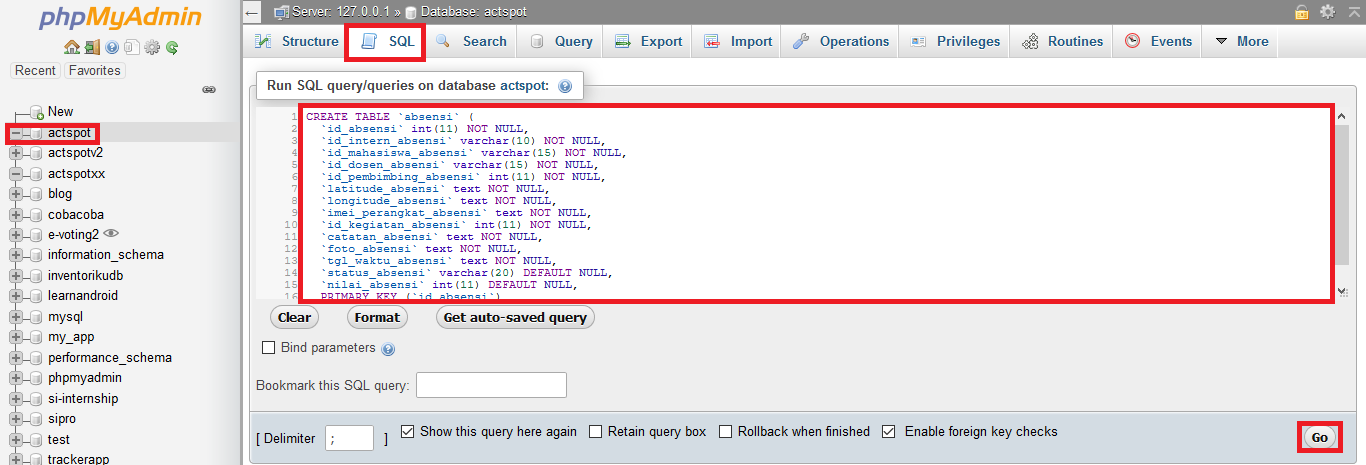
\includegraphics[width=1\textwidth]{figures/database/database4.png}
\end{figure}

\noindent
Selanjutnya kita akan membuat tabel detail\_absensi. Caranya sama dengan sebelumnya, lalu ketikan script berikut dan klik Go untuk mengeksekusinya.

\begin{lstlisting}[language=SQL]
CREATE TABLE `detail_absensi` (
  `id_absensi` int(11) NOT NULL AUTO_INCREMENT,
  `id_mahasiswa_dt_absensi` varchar(15) NOT NULL,
  `id_absensi_dt_absensi` int(11) NOT NULL,
  `pergeseran_absensi` text NOT NULL,
)
\end{lstlisting}

\noindent
Setelah itu kita akan membuat trigger pergeseran\_absensi untuk mengukur pergeseran antara objek dengan lokasi yang telah ditentukan. Caranya sama dengan sebelumnya, lalu ketikan script berikut dan klik Go untuk mengeksekusinya.

\begin{lstlisting}[language=SQL]
DELIMITER $$
CREATE TRIGGER `pergeseran_absensi` AFTER INSERT ON `absensi` FOR EACH ROW INSERT INTO detail_absensi (id_intern_dt_absensi,id_mahasiswa_dt_absensi,id_absensi_dt_absensi, pergeseran_absensi)
    SELECT NEW.id_intern_absensi
         , NEW.id_mahasiswa_absensi 
         , NEW.id_absensi 
         , hitung_pergeseran(p.lat_pembimbing_perusahaan ,p.long_pembimbing_perusahaan ,NEW.latitude_absensi,NEW.longitude_absensi)
      FROM pembimbing_perusahaan p
      LIMIT 1
$$
DELIMITER ;
\end{lstlisting}

\noindent
Selanjutnya kita akan membuat tabel detail\_intern. Caranya sama dengan sebelumnya, lalu ketikan script berikut dan klik Go untuk mengeksekusinya.

\begin{lstlisting}[language=SQL]
CREATE TABLE `detail_intern` (
  `id_intern_dt_intern` int(11) NOT NULL,
  `id_mahasiswa_dt_intern` varchar(15) NOT NULL,
  `id_dosen_dt_intern` varchar(15) NOT NULL,
  `lama_internship` int(11) NOT NULL,
  `surat_intern` text NOT NULL,
  `id_pembimbing_dt_intern` int(11) DEFAULT NULL,
  `latitude_perusahaan` text,
  `longitude_perusahaan` text,
  `foto_perusahaan` text,
  `status_perusahaan` varchar(20) DEFAULT NULL
)
\end{lstlisting}

\noindent
Setelah itu, kita akan membuat tabel dosen. Caranya sama dengan sebelumnya, lalu ketikan script berikut dan klik Go untuk mengeksekusinya.

\begin{lstlisting}[language=SQL]
CREATE TABLE `dosen` (
  `id_dosen` varchar(15) NOT NULL,
  `nama_dosen` varchar(50) NOT NULL,
  `id_prodi_dosen` varchar(10) NOT NULL,
  `kontak_dosen` text NOT NULL,
  `foto_dosen` text,
  PRIMARY KEY (`id_dosen`)
)
\end{lstlisting}

\noindent
Selanjutnya kita akan membuat tabel intern. Caranya sama dengan sebelumnya, lalu ketikan script berikut dan klik Go untuk mengeksekusinya.

\begin{lstlisting}[language=SQL]
CREATE TABLE `intern` (
  `id_intern` int(11) NOT NULL AUTO_INCREMENT,
  `id_koor_intern` varchar(15) NOT NULL,
  `status_intern` varchar(15) NOT NULL,
  `tgl_mulai_intern` datetime DEFAULT NULL,
  `tgl_akhir_intern` datetime DEFAULT NULL,
  PRIMARY KEY (`id_intern`)
)
\end{lstlisting}

\noindent
Setelah itu, kita akan membuat tabel kegiatan. Caranya sama dengan sebelumnya, lalu ketikan script berikut dan klik Go untuk mengeksekusinya.

\begin{lstlisting}[language=SQL]
CREATE TABLE `kegiatan` (
  `id_kegiatan` int(11) NOT NULL AUTO_INCREMENT,
  `nama_kegiatan` varchar(50) NOT NULL,
  PRIMARY KEY (`id_kegiatan`)
)
\end{lstlisting}

\noindent
Selanjutnya kita akan membuat tabel mahasiswa. Caranya sama dengan sebelumnya, lalu ketikan script berikut dan klik Go untuk mengeksekusinya.

\begin{lstlisting}[language=SQL]
CREATE TABLE `mahasiswa` (
  `id_mahasiswa` varchar(15) NOT NULL,
  `nama_mahasiswa` varchar(50) NOT NULL,
  `kelas_mahasiswa` varchar(5) NOT NULL,
  `id_prodi_mahasiswa` varchar(10) NOT NULL,
  `angkatan_mahasiswa` varchar(5) NOT NULL,
  `foto_mahasiswa` text,
  `kontak_mahasiswa` varchar(25) NOT NULL,
  `kode_otp` varchar(11) DEFAULT NULL,
  PRIMARY KEY (`id_mahasiswa`)
)
\end{lstlisting}

\noindent
Setelah itu, kita akan membuat tabel notifikasi. Caranya sama dengan sebelumnya, lalu ketikan script berikut dan klik Go untuk mengeksekusinya.

\begin{lstlisting}[language=SQL]
CREATE TABLE `notifikasi` (
  `id_intern_notifikasi` int(11) NOT NULL,
  `id_mahasiswa_notifikasi` varchar(15) NOT NULL,
  `id_dosen_notifikasi` varchar(15) NOT NULL,
  `id_pembimbing_notifikasi` int(11) NOT NULL,
  `pesan_notifikasi` text NOT NULL,
  `tgl_waktu_notifikasi` datetime NOT NULL
)
\end{lstlisting}

\noindent
Selanjutnya kita akan membuat tabel pembimbing\_perusahaan. Caranya sama dengan sebelumnya, lalu ketikan script berikut dan klik Go untuk mengeksekusinya.

\begin{lstlisting}[language=SQL]
CREATE TABLE `pembimbing_perusahaan` (
  `id_pembimbing` int(11) NOT NULL AUTO_INCREMENT,
  `nama_pembimbing` varchar(50) NOT NULL,
  `nama_perusahaan_perusahaan` text NOT NULL,
  `lat_pembimbing_perusahaan` text NOT NULL,
  `long_pembimbing_perusahaan` text NOT NULL,
  `kontak_pembimbing` varchar(25) NOT NULL,
  `foto_pembimbing` text,
  PRIMARY KEY (`id_pembimbing`)
)
\end{lstlisting}

\noindent
Setelah itu, kita akan membuat tabel prodi. Caranya sama dengan sebelumnya, lalu ketikan script berikut dan klik Go untuk mengeksekusinya.

\begin{lstlisting}[language=SQL]
CREATE TABLE `prodi` (
  `id_prodi` varchar(10) NOT NULL,
  `nama_prodi` varchar(50) NOT NULL,
  PRIMARY KEY (`id_prodi`)
)
\end{lstlisting}

\noindent
Selanjutnya kita akan membuat tabel user. Caranya sama dengan sebelumnya, lalu ketikan script berikut dan klik Go untuk mengeksekusinya.

\begin{lstlisting}[language=SQL]
CREATE TABLE `user` (
  `id_user` varchar(15) NOT NULL,
  `username` varchar(20) NOT NULL,
  `password` text NOT NULL,
  `status_user` varchar(15) NOT NULL,
  `role_user` varchar(15) NOT NULL
)
\end{lstlisting}

\noindent
Sehingga hasilnya akhirnya terbentuk beberapa tabel yang dibutuhkan.

\begin{figure}[H]
\centering
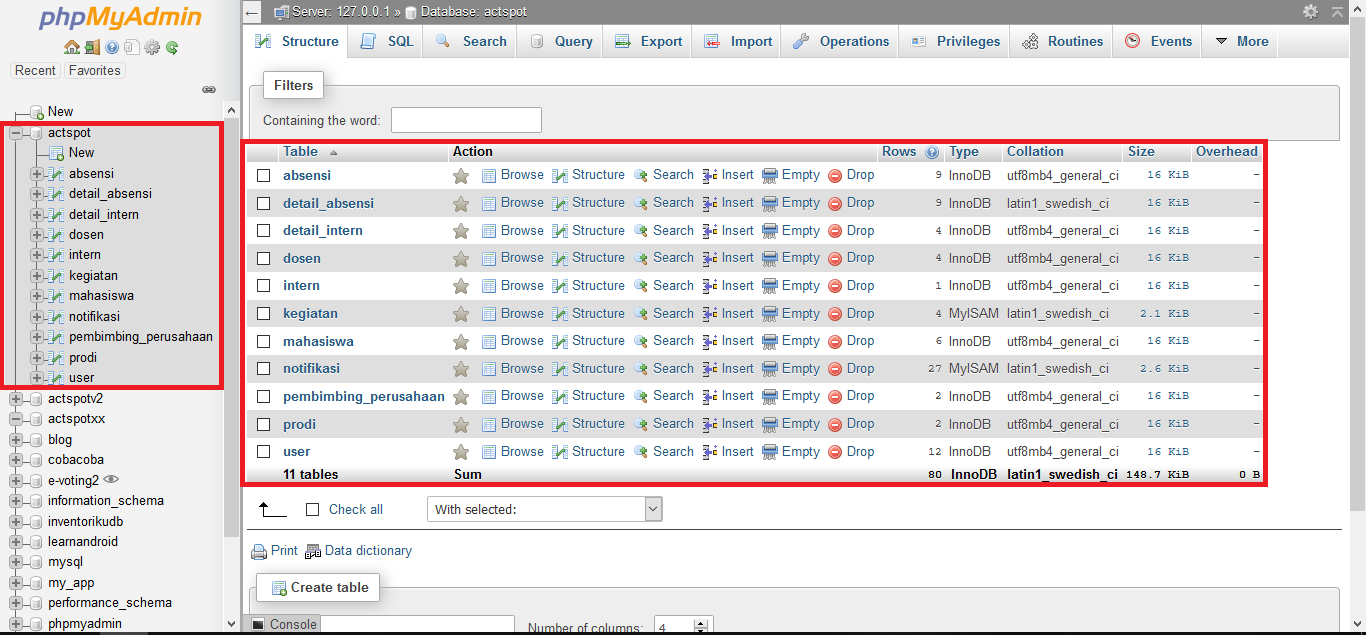
\includegraphics[width=10cm]{figures/database/database5.png}
\end{figure}